\documentclass[12pt, titlepage, twoside]{amsart}

\usepackage[a4paper, margin=1in]{geometry}
\usepackage{amsmath}
\usepackage[foot]{amsaddr}
\usepackage{enumitem}
\usepackage[dvipsnames]{xcolor}
\usepackage{parskip}
\usepackage{esvect}
\usepackage{url}
\usepackage{graphicx}
\usepackage{minted}
\usepackage{hyperref}

\newcommand{\R}{\ensuremath{\mathbb R}}
\newcommand{\Z}{\ensuremath{\mathbb Z}}
\newcommand{\N}{\ensuremath{\mathbb N}}

\graphicspath{{../img/}}
\setminted{linenos, breaklines}
\hypersetup{
  colorlinks=true,
  citecolor=BurntOrange,
  linkcolor=Rhodamine,
  urlcolor=MidnightBlue
}

\raggedright

\begin{document}

\title[ScottyRank.jl]{ScottyRank.jl: An Implementation of PageRank \& HITS}

\author{Siyuan Chen}
\author{Michael Zhou}
\email{siyuanc2@andrew.cmu.edu}
\email{mhzhou@andrew.cmu.edu}
\date{November 2021}

\begin{abstract}
We present \href{https://github.com/mzhou08/ScottyRank.jl}{ScottyRank.jl},
a Julia implementation of the PageRank algorithm and one of its successors, the HITS algorithm.
Famously used by Google, PageRank, as well as its variations,
models a network of interest (such as the Internet) as a simple directed graph and produces relative rankings
of the vertices that roughly translate to the vertices’ levels of relevance and importance.

In this paper, we first introduced the mathematical background for the two algorithms.
We then outlined the core algorithmic insights of both PageRank and HITS and expressed them in matrix form.
Using code segments, we presented our implementation of the two algorithms.
Finally, we ran the two algorithms on the Wikipedia PageRank network and analyzed the outputs.~\cite{pagerank}
We included the source code in the Appendix.
\end{abstract}

\maketitle

\tableofcontents

\clearpage

\section{Background}

\subsection{Linear Algebra}

\subsubsection{Definitions}

Positive matrices are defined as matrices with positive entries.

Markov matrices are defined as square matrices with nonnegative entries and column sum $1$ across all of its columns.
Note that for a $n\times n$ matrix $M$, the latter condition is equivalent to $M^T\vec{1} = \vec{1}$,
where $\vec{1}\in\R^n$ has all ones as components.

Positive Markov matrices are defined as, well, positive Markov matrices.

\subsubsection{Facts}

(Perron-Frobenius theorem)
Let $A$ be a positive square matrix.
Let $\lambda_1$ be $A$'s maximum eigenvalue in terms of absolute values.
Then $\lambda_1$ is positive and has algebraic (and subsequently geometric) multiplicity $1$.~\cite{perron}

Let $M$ be a Markov matrix.
Let $\lambda_1$ be $M$'s maximum eigenvalue in terms of absolute values.
Then $\lambda_1 = 1$.~\cite{strang}

Let $M'$ be a positive Markov matrix.
Let $\lambda_1$ be $M'$'s maximum eigenvalue in terms of absolute values.
Then $\lambda_1 = 1$ and has algebraic (and subsequently geometric) multiplicity $1$.

\subsubsection{Usage}

Let $M$ be a $n\times n$ Markov matrix.
Then $M$ specifies a dicrete memoryless transition process between $n$ states, namely the process where
\[
  \left(\forall (t, i, j)\in\N\times[n]\times[n]\right)
  \left[\Pr(\text{state }i\text{ at time }t + 1\mid \text{state }j\text{ at time }t) = M_{ij}\right].
\]

Let $\vec{v}\in\R^n$ such that $\vec{v}$ has nonnegative components and $\vec{v}^T\vec{1} = 1$ (a stochastic vector).
Then $\vec{v}$ specifies an (initial) discrete probability distribution over the $n$ states, namely the distribution where
\[
  (\forall i\in[n])
  [\Pr(\text{state }i\text{ at time }0) = \vec{v}_i].
\]

Then the probability distribution over the $n$ states after $t$ steps of the transition process specified by $M$ is precisely $M^t\vec{v}$,
or equivalently
\[
  (\forall (t, i)\in\N\times[n])
  \left[\Pr(\text{state }i\text{ at time }t) = \left(M^t\vec{v}\right)_i\right].
\]

\subsection{Graph Theory}

\subsubsection{Definitions}

A simple directed graph is defined as an unweighted directed graph without self-referential edges or multiple edges
between the same origin destination pair.

For a simple directed graph with $n$ vertices, the adjacency matrix $\mathcal{A}$ is defined to be
the $n\times n$ matrix where
\[
  (\forall (i, j)\in[n]\times[n])\left(A_{ij} = 
    \begin{cases}
      1 & \text{there is an edge to $i$ from $j$} \\
      0 & \text{otherwise}
    \end{cases}
  \right).
\]

\subsubsection{Facts}

For a simple directed graph with $n$ vertices and its adjacency matrix $\mathcal{A}$,
\begin{align*}
  (\forall j\in[n])&
  \left[\text{number of outgoing neighbors from vertex $j$} = \mathrm{out}(j) = (\mathcal{A}_{*j})^T\vec{1}\right] \\
  (\forall i\in[n])&
  \left[\text{number of incoming neighbors to vertex $i$} = \mathrm{in}(i) = (\mathcal{A}_{i*})^T\vec{1}\right].
\end{align*}

\section{Algorithms}

\subsection{The Network Model}

Both algorithms, PageRank and HITS, model the network of interest as a simple directed graph with websites as vertices
and links as edges.
This implies that there will be no self-referential links, no duplicate links between the same origin
and destination pair, and no priority difference between links.

\subsection{PageRank}

\subsubsection{The random walk}

PageRank models the behavior of a typical web surfer as a damped random walk.~\cite{pagerank}

\begin{enumerate}
  \item The surfer starts out by visiting a random site out of all sites with equal probability.
  \item At every step, the surfer has a probability $\lambda$ of continuing surfing and a complementary
    $1 - \lambda$ probability of losing interest, for a predetermined $\lambda$.
  
    \begin{enumerate}
      \item If the surfer continues \ldots

        \begin{enumerate}
          \item \ldots and there are links exiting the current site, the surfer
            clicks on a random link (and visits the site it points to) out of those links with equal probability.
          \item \ldots and there aren't any links exiting the current site, the surfer simply
            visits a random site out of all other sites with equal probability.
        \end{enumerate}

      \item If the surfer loses interest, they simply visits a random site out of all sites with equal probability.
    \end{enumerate}

\end{enumerate}

To best model a typical surfer's probability of continuing surfing, $\lambda$, also known as the damping factor,
is empirically determined to be around $0.85$.

\subsubsection{Matrix representation}

Let $n$ be the number of websites in the network of interest.
Let $\mathcal{A}$ be the adjacency matrix for the network of interest.
Let $\langle\vec{v}_{t}\rangle_{t\in\N}$ be the probability distributions describing the
website the surfer is visiting at time $t$.
Let $M$ be the transition matrix for the random walk process.

Then $\vec{v}_0 = \vec{1} / n$,
$M$ is the $n\times n$ matrix where
\[
  (\forall (i, j)\in[n]\times[n])
  \left[
  M_{ij} =
  \begin{cases}
    \frac{\lambda}{\mathrm{out}(j)} + \frac{1 - \lambda}{n}
    & \mathcal{A}_{ij} = 1 \\
    \frac{1 - \lambda}{n}
    & \mathcal{A}_{ij} = 0\wedge\mathrm{out}(j) > 0 \\
    \frac{\lambda}{n - 1} + \frac{1 - \lambda}{n}
    & i \neq j\wedge\mathrm{out}(j) = 0 \\
    \frac{1 - \lambda}{n}
    & i = j\wedge\mathrm{out}(j) = 0
  \end{cases}
  \right],
\]
and
\[
  (\forall t\in\N)\left(\vec{v}_t = M^t\vec{v}_0\right).
\]

Note that in this case $M$ is a positive Markov matrix, assuming reasonable $\lambda$.

\subsubsection{Definition}

The PageRank score for a given website in the network of interest is defined as the probabilty of a typical surfer
visiting that website after an indefinitely long damped random walk.
In matrix form,
\[
  (\forall i\in[n])
  \left[\mathrm{PageRank}(i) = \lim_{t\to\infty}(\vec{v}_t)_i = \lim_{t\to\infty}\left(M^t\vec{v}_0\right)_i\right].
\]

Note that the limits exist: convergence is guaranteed as $M$ has a unique maximal eigenvalue of $1$ and thus an steady
attracting state.

\subsection{HITS}

\subsubsection{Authorities and hubs}

Due to PageRank's algorithmic design, a given website's PageRank score determined mostly by the scores of its
incoming neighbors.
Consequently, PageRank tends to underestimate the importance of websites similar to ``web directories'', i.e., those
with few significant incoming neighbors yet many significant outgoing neighbors.

To address this issue, HITS (Hyperlink-Induced Topic Search) introduces Authority and Hub scores, which measure
a given website's tendencies to be refered to by others and to refer to others, respectively.
Note that the two metrics are not ``mutually exclusive''; a website like Wikipedia can have both a high Authority score
and a high Hub score.

Specifically, Authority and Hub scores are recursively defined: a website's Authority score is determined by
the Hub scores of its incoming neighbors and its Hub score is determined by the Authority scores of its outgoing
neighbors.~\cite{hits}~\cite{tanase}

\subsubsection{Matrix representation}

Let $n$ be the number of websites in the network of interest.
Let $\mathcal{A}$ be the adjacency matrix for the network of interest.
Let $\langle\vec{a}_t\rangle_{t\in\N}$ and $\langle\vec{h}_t\rangle_{t\in\N}$ be the (pre-normalization)
Authority and Hub scores for the $n$ websites at time $t$.

Then $\vec{a}_0 = \vec{h}_0 = \vec{1}$ and
\[
  (\forall t\in\N)
  \left[
    \left(\vec{a}_{t + 1}, \vec{h}_{t + 1}\right) = \left(\mathcal{A}\vec{h}_t, \mathcal{A}^T\vec{a}_t\right)
  \right].
\]

\subsubsection{Definition} The Authority and Hub scores for a given website in the network of interest is defined
as the respective scores after indefinitely many iterations.
In matrix form,
\[
  (\forall i\in[n])
  \left[
    \left(\mathrm{Authority}(i), \mathrm{Hub}(i)\right) =
    \lim_{t\to\infty}
    \left((\vec{a}_t)_i, (\vec{h}_t)_i\right)
  \right].
\]

To guarantee convergence, the Authority and Hub scores are normalized.
Our implementation performs normalization after every iteration.
This means
\[
  (\forall t\in\N)
  \left[
    \lVert(\vec{a}_t)'\rVert = \lVert(\vec{h}_t)'\rVert = 1
  \right]
\]
where
\[
  (\forall t\in\N)
  \left[
    (\vec{a}_t)' = \frac{\vec{a}_t}{\lVert\vec{a}_t\rVert}
    \wedge
    (\vec{h}_t)' = \frac{\vec{h}_t}{\lVert\vec{h}_t\rVert}
  \right].
\]

\section{Implementation}

\subsection{Structs}

We define two structs, \mintinline{julia}{Vertex} and \mintinline{julia}{Graph}, to represent
the vertices and the graph itself in our simple directed graph model for the network of interest.

Note that to align with Julia conventions, we use 1-based indexing.~\cite{julialang}

\begin{minted}{julia}
# export Vertex, Graph

struct Vertex
  index::UInt32
  in_neighbors::Vector{UInt32}
  out_neighbors::Vector{UInt32}
end

struct Graph
  num_vertices::UInt32
  vertices::Vector{Vertex}
end
\end{minted}

\subsection{Input}

We define three functions,
\mintinline{julia}{read_graph}, \mintinline{julia}{read_edge_list}, and \mintinline{julia}{read_adjacency_list},
to read and construct graphs from text files.
We expose \mintinline{julia}{read_graph} to the client with the option to specify the type of the input file and
whether or not the input file uses 0-based indexing.

Edge list files follow the following format:

\begin{minted}{julia}
[num_nodes] [num_edges]
[index_from] [index_to] # repeats [num_edges] times
...                     # in total
\end{minted}

Adjacency list files follow the following format:

\begin{minted}{julia}
[num_nodes]
[index_to_1] [index_to_2] ... [index_to_m] # repeats [num_nodes] times
...                                        # in total
\end{minted}

The code for
\mintinline{julia}{read_graph},
\mintinline{julia}{read_edge_list}, and \mintinline{julia}{read_adjacency_list} can be found in the
Appendix.

\subsection{PageRank}

We divide the PageRank algorithm into three steps:

\begin{enumerate}
  \item Generating the transition matrix: \mintinline{julia}{pagerank_matrix}.
  \item Running the transition process: \mintinline{julia}{pagerank_iteration}, \mintinline{julia}{pagerank_epsilon}.
  \item Returning the desired output: \mintinline{julia}{pagerank_print}, \mintinline{julia}{pagerank}.
\end{enumerate}

\subsubsection{Generating the transition matrix}

The function \mintinline{julia}{pagerank_matrix} generates a Markov matrix $M$ that specifies the transition
probabilities of the PageRank transition process.

We first compute the entries in $M$ prior to damping, casing on whether the origin vertex is a ``sink''
(no outgoing neighbors), and then apply the damping at the end.

\begin{minted}{julia}
function pagerank_matrix(graph::Graph, damping::Float64)
  M = zeros(Float64, (graph.num_vertices, graph.num_vertices))
  for vertex in graph.vertices
    num_out_neighbors = length(vertex.out_neighbors)
    if num_out_neighbors == 0
      for index_to in 1:graph.num_vertices
        M[index_to, vertex.index] = 1 / (graph.num_vertices - 1)
      end
      M[vertex.index, vertex.index] = 0
    else
      for index_to in vertex.out_neighbors
        M[index_to, vertex.index] = 1 / num_out_neighbors
      end
    end
  end
  map(x -> damping * x + (1 - damping) / graph.num_vertices, M)
end
\end{minted}

\subsubsection{Running the transition process}

The functions \mintinline{julia}{pagerank_iteration} and \mintinline{julia}{pagerank_epsilon} both generate
an initial stochastic vector and then carry out the transition process using the transition matrix.

\mintinline{julia}{pagerank_iteration} runs the process for a given number of iterations.

\begin{minted}{julia}
function pagerank_iteration(num_vertices::UInt32, M::Matrix{Float64}, num_iterations::UInt32)
  M_pwr = Base.power_by_squaring(M, num_iterations) 
  M_pwr * (ones(Float64, num_vertices) / num_vertices)
end
\end{minted}

\mintinline{julia}{pagerank_epsilon} runs the process until the norm of the difference vector
is smaller than a given threshold, or until
$\left\lVert\vec{v}_{k + 1} - \vec{k}\right\rVert < \epsilon$.

\begin{minted}{julia}
function pagerank_epsilon(num_vertices::UInt32, M::Matrix{Float64}, epsilon::Float64)
  prev = ones(Float64, num_vertices) / num_vertices
  curr = M * prev
  while norm(prev - curr) > epsilon
    prev, curr = curr, M * curr
  end
  curr
end
\end{minted}

\subsubsection{Returning the desired output}

We expose two functions to the client: \mintinline{julia}{pagerank} and \mintinline{julia}{pagerank_print}.

\mintinline{julia}{pagerank} calculates the PageRank scores for the input \mintinline{julia}{graph},
with the option to specify the damping factor and the transition mode.

\begin{minted}{julia}
# export pagerank_print, pagerank

function pagerank(graph::Graph;
    damping::Float64=0.85, modeparam::Tuple{String, Union{Int64, UInt32, Float64}}=("iter", 10))
  if damping < 0 || damping > 1
    error("invalid damping")
  end
  M = pagerank_matrix(graph, damping)
  if modeparam[1] == "iter"
    if !(isinteger(modeparam[2])) || modeparam[2] < 0
      error("invalid param")
    end
    pagerank_iteration(graph.num_vertices, M, UInt32(modeparam[2]))
  elseif modeparam[1] == "epsi"
    if modeparam[2] <= 0
      error("invalid param")
    end
    pagerank_epsilon(graph.num_vertices, M, Float64(modeparam[2]))
  else
    error("invalid mode")
  end
end
\end{minted}

\mintinline{julia}{pagerank_print} pretty-prints the PageRank scores along with relevant information about the top
vertices for the input \mintinline{julia}{graph} and scores \mintinline{julia}{pg}.

The code for \mintinline{julia}{pagerank_print} can be found in the Appendix.

\subsection{HITS}

Similarly, we divide the HITS algorithm into three steps:

\begin{enumerate}
  \item Generating the transition matrix: \mintinline{julia}{hits_matrix}.
  \item Running the transition process: \mintinline{julia}{hits_update}, \mintinline{julia}{hits_iteration},
    \mintinline{julia}{hits_epsilon}.
  \item Returning the desired output: \mintinline{julia}{hits_print}, \mintinline{julia}{hits}.
\end{enumerate}

\subsubsection{Generating the transition matrix}

The transition matrices for the hits algorithm are simply the adjacency matrix and its transpose.

\begin{minted}{julia}
function hits_matrix(graph::Graph)
  A = zeros(Float64, (graph.num_vertices, graph.num_vertices))
  for vertex in graph.vertices
    for index_to in vertex.out_neighbors
      A[index_to, vertex.index] = 1
    end
  end
  A
end
\end{minted}

\subsubsection{Running the transition process}

The function \mintinline{julia}{hits_update} computes the normalized new Authority and Hub scores from the
previous Authority and Hub scores and the two transition matrices

\begin{minted}{julia}
function hits_update(A::Matrix{Float64}, H::Matrix{Float64}, a::Vector{Float64}, h::Vector{Float64})
  normalize(A * h), normalize(H * a)
end
\end{minted}

The functions \mintinline{julia}{hits_iteration} and \mintinline{julia}{hits_epsilon}
both generate the initial Authority and Hub scores and then carry out the transition process using the update function.

\mintinline{julia}{hits_iteration} runs the process for a given number of iterations.

\begin{minted}{julia}
function hits_iteration(num_vertices::UInt32, A::Matrix{Float64}, H::Matrix{Float64}, num_iterations::UInt32)
  a, h = ones(Float64, num_vertices), ones(Float64, num_vertices)
  for _ in 1:num_iterations
    a, h = hits_update(A, H, a, h)
  end
  a, h
end
\end{minted}

\mintinline{julia}{hits_epsilon} runs the process until the norms of both difference vectors are smaller than 
the given threshold, or until
$\left\lVert
  \vec{a}_{k + 1} - \vec{a}_k
\right\rVert < \epsilon
\wedge
\left\lVert
  \vec{h}_{k + 1} - \vec{h}_k
\right\rVert < \epsilon$.

\begin{minted}{julia}
function hits_epsilon(num_vertices::UInt32, A::Matrix{Float64}, H::Matrix{Float64}, epsilon::Float64)
  prev_a, prev_h = ones(Float64, num_vertices), ones(Float64, num_vertices)
  curr_a, curr_h = hits_update(A, H, prev_a, prev_h)
  while norm(prev_a - curr_a) > epsilon || norm(prev_h - curr_h) > epsilon
    prev_a, prev_h, (curr_a, curr_h) = curr_a, curr_h, hits_update(A, H, curr_a, curr_h)
  end
  curr_a, curr_h
end
\end{minted}

\subsubsection{Returning the desired output}

We expose two functions to the client: \mintinline{julia}{hits} and \mintinline{julia}{hits_print}

\mintinline{julia}{hits} calculates the Authority and Hub scores for the input \mintinline{julia}{graph},
with the option to specify the transition mode.

\begin{minted}{julia}
# export hits_print, hits

function hits(graph::Graph;
    modeparam::Tuple{String, Union{Int64, UInt32, Float64}}=("iter", 10))
  A = hits_matrix(graph)
  H = copy(transpose(A))
  if modeparam[1] == "iter"
    if !(isinteger(modeparam[2])) || modeparam[2] < 0
      error("invalid param")
    end
    hits_iteration(graph.num_vertices, A, H, UInt32(modeparam[2]))
  elseif modeparam[1] == "epsi"
    if modeparam[2] <= 0
      error("invalid param")
    end
    hits_epsilon(graph.num_vertices, A, H, Float64(modeparam[2]))
  else
    error("invalid mode")
  end
end
\end{minted}

\mintinline{julia}{hits_print} pretty-prints the Authority and Hub scores along with relevant information
about the top vertices for the input \mintinline{julia}{graph} and scores \mintinline{julia}{a} and \mintinline{julia}{h}.

The code for \mintinline{julia}{hits_print} can be found in the Appendix.

\subsection{Output}

We offer two ways of exporting the \mintinline{julia}{graph} struct: \mintinline{julia}{generate_adjacency_matrix}
and \mintinline{julia}{generate_adjacency_list}, which, well, generate the \mintinline{julia}{graph}'s
adjacency matrix and adjacency list, respectively.

The code for \mintinline{julia}{generate_adjacency_matrix} and \mintinline{julia}{generate_adjacency_list} and be
found in the Appendix.

\section{Example}

\subsection{The Wikipedia PageRank graph}

Shown below is a recreation of the medium-sized network with 11 websites displayed in
the Wikipedia article on PageRank.~\cite{pagerank}\cite{snap}
We will run both PageRank and HITS on this network.

\begin{center}
  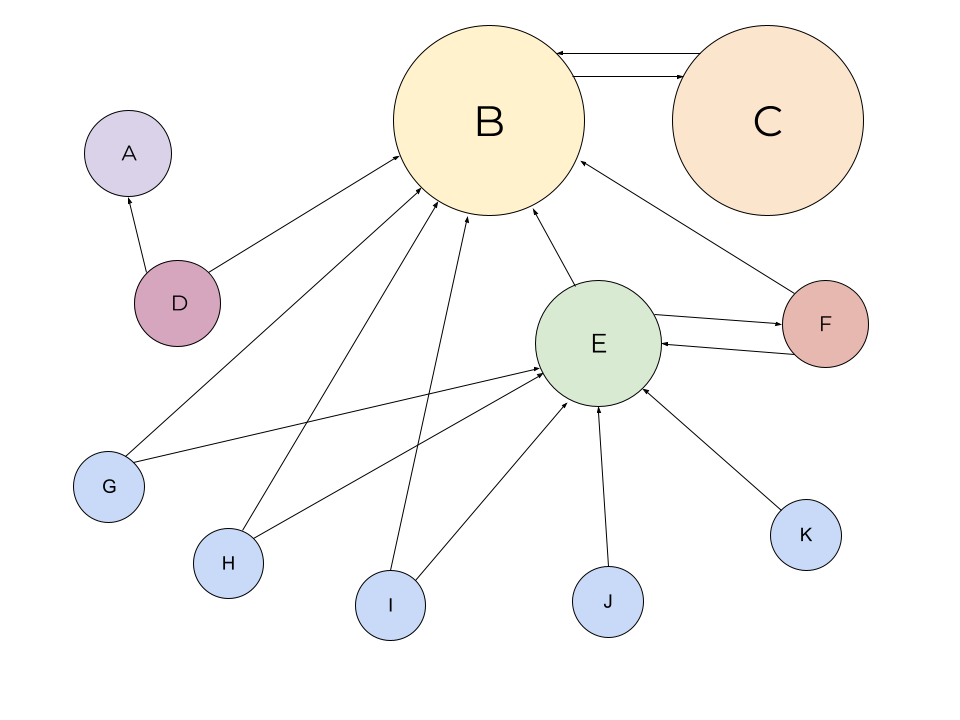
\includegraphics[scale = 0.4]{wikipedia.png}
\end{center}


\subsection{PageRank}

\subsubsection{Expectations}

We expect websites B and C to have the highest PageRank scores
because virtually every website links to it, either directly or through other websites such as E.

We also expect E to have a fairly high PageRank score because there are many websites linking to it.

Finally, we expect websites G, H, I, J, and K to have the lowest PageRank scores because they only have outgoing links.

\subsubsection{Results}

We run the following commands to apply PageRank on the network.

\begin{minted}[linenos=false]{julia}
$ julia
julia> using ScottyRank
julia> G = read_graph("data/medium-el.txt", filetype = "el")
julia> pg = pagerank(G, modeparam=("epsi", 0.01))
julia> pagerank_print(G, pg, num_lines=11)
 - -  vall | - - index | - -    in | - -   out |
--- pagerank ---
    0.3824 |         2 |         7 |         1 | # B
    0.3467 |         3 |         1 |         1 | # C
    0.0811 |         5 |         6 |         3 | # E
    0.0392 |         4 |         1 |         2 | # D
    0.0392 |         6 |         1 |         2 | # F
    0.0303 |         1 |         1 |         0 | # A
    0.0162 |         7 |         0 |         2 | # G
    0.0162 |         8 |         0 |         2 | # H
    0.0162 |         9 |         0 |         2 | # I
    0.0162 |        10 |         0 |         1 | # J
    0.0162 |        11 |         0 |         1 | # K
\end{minted}

The first column lists the calculated PageRank score and
the second lists the index of the website with that score.
The ``in'' column displays the number of incoming links to the corresponding website.
Similarly, the ``out'' column displays the number of outgoing edges from the corresponding website.

We see that, as expected, websites B and C have the highest PageRank scores by far,
and E has the highest score of the remaining websites.
Additionally, we see the websites G, H, I, J, and K share the same lowest PageRank score.

\subsection{HITS}

\subsubsection{Expectations}

Recall the core concept of HITS:
websites linked by websites with high Hub scores will have high Authority scores;
websites linking to websites with high Authority scores will have high Hub scores.

With this in mind, we expect that websites B and E to have the highest Authority scores
simply because they have the greatest number of websites linking to them.

However, since B does not link towards many other Authorities, its Hub score should be low.
But E links to B, which has a high Authority score, so we expect the Hub score of E to be above average.

Similarly, the Hub score of C should be relatively high since it links to B, but the Authority score of
C should be low because B does not have a high Hub score.

Finally, we expect the Authority scores of G, H, I, J, and K all to be very low
because no websites link towards them.
However, their Hub scores should be relatively high because they point to
one or both of the highest Authority websites, namely B and E.

\subsubsection{Results}

We run the following commands to apply HITS on the network.

\begin{minted}[linenos=false]{julia}
$ julia
julia> using ScottyRank
julia> G = read_graph("data/medium-el.txt", filetype = "el")
julia> a, h = hits(G, modeparam=("epsi", 0.01))
julia> hits_print(G, a, h, num_lines=11)
 - -  vall | - - index | - -    in | - -   out |
--- authority ---
    0.7567 |         2 |         7 |         1 | # B
    0.6370 |         5 |         6 |         3 | # E
    0.0880 |         4 |         1 |         2 | # D
    0.0880 |         6 |         1 |         2 | # F
    0.0784 |         1 |         1 |         0 | # A
    0.0000 |         3 |         1 |         1 | # C
    0.0000 |         7 |         0 |         2 | # G
    0.0000 |         8 |         0 |         2 | # H
    0.0000 |         9 |         0 |         2 | # I
    0.0000 |        10 |         0 |         1 | # J
    0.0000 |        11 |         0 |         1 | # K
--- hub ---
    0.4259 |         6 |         1 |         2 | # F
    0.4259 |         7 |         0 |         2 | # G
    0.4259 |         8 |         0 |         2 | # H
    0.4259 |         9 |         0 |         2 | # I
    0.2836 |         5 |         6 |         3 | # E
    0.2544 |         4 |         1 |         2 | # D
    0.2306 |         3 |         1 |         1 | # C
    0.1952 |        10 |         0 |         1 | # J
    0.1952 |        11 |         0 |         1 | # K
    0.0000 |         2 |         7 |         1 | # B
    0.0000 |         1 |         1 |         0 | # A
\end{minted}

Similar to \mintinline{julia}{pagerank_print}, the first column
of the first table lists the Authority score
and the first column of the second table lists the Hub scores.
The ``in'' column displays the number of incoming links to the corresponding website,
and the ``out'' column displays the number of outgoing edges from the corresponding website.

As expected, the Authority scores of B and E are the highest, with C having a low Authority score.
The vertices G, H, I, J, and K have Authority scores of 0 because no vertices point to them.

Furthermore, we see that the Hub scores are also calculated as predicted:
the Hub score of F is the highest because F links towards both B and E,
the two vertices with the highest authority scores. G, H, I also
have very high Hub scores. However, J and K have lower Hub scores because they only link to one of the main Authorities.

\bibliographystyle{acm}
\bibliography{refs}

\appendix

\section{Links}

The project repository can be found at
\href{https://github.com/mzhou08/ScottyRank.jl}{\texttt{https://github.com/mzhou08/ScottyRank.jl}}.

\section{Code}

\inputminted{julia}{../src/ScottyRank.jl}

\end{document}
